\newpage
\section{DQN 改进算法}

\subsection{倒立摆 环境}
倒立摆 (Inverted Pendulum) 环境, 有一个处于随机位置的倒立摆, 其动作空间是连续的. 

\begin{figure}[!htb]
    \centering
    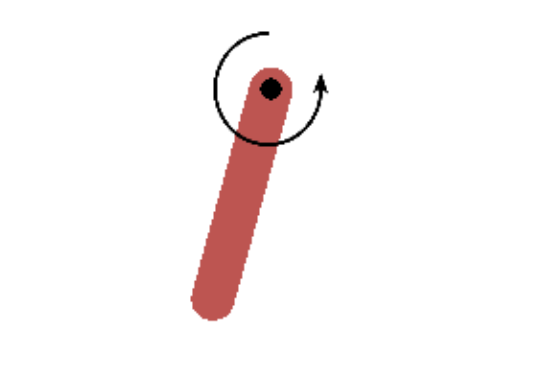
\includegraphics[width=0.618\linewidth]{pic/RL8/倒立摆.png}
    \caption{倒立摆}
\end{figure}

其奖励函数是
\begin{align*}
    -(\theta^2 + 0.1 \dot{\theta}^2 +0.001 a^2)
\end{align*}
其中 $\theta$ 是倒立摆的角度, $a$ 是给予的力矩. 倒立摆向上保持直立不动时奖励函数为 0, 其他位置奖励函数为负, 没有终止状态, 200 步后自动结束. 动作空间就是力矩的值, 是连续的. 

\begin{table}[!htb]
    \centering
    \caption{倒立摆 环境状态空间与动作空间}
    \begin{tabular}[c]{ccc}\toprule
        意义 & 最小值 & 最大值 \\ \midrule
        $\cos \theta$ & $-1.0$ & $1.0$ \\
        $\sin \theta$  & $-1.0$ & $1.0$ \\
        $\dot \theta$  & $-8.0$ & $8.0$ \\ \cmidrule{1-1}
        力矩 $a$ & $-2.0$ & $2.0$   \\
        \bottomrule
    \end{tabular}
\end{table}


\subsection{Double DQN}
普通的 DQN 通常会对 $Q$ 有过高的估计 (overestimation). 传统 DQN 误差目标为,
\begin{align*}
    &r+\gamma \max_{a'} Q_{\omega^-} (s', a')\\
    =&r+ \gamma Q_{\omega^-}\left( s', \argmax_{a'} Q_{\omega^-} (s', a') \right)
\end{align*}
可看做是先选取最优动作 $a^* = \argmax_{a'} Q_{\omega^-} (s', a')$, 然后计算动作对应的价值 $Q_{\omega^-}(s', a^*)$. 但是因为计算时用的都是同一套神经网络, 会有正负向误差, 而每次取 $\max$ 会导致误差正向积累. 

例如, 假设在状态 $s'$ 下任意动作的价值都是 0, i.e.  $\forall i,\ Q(s', a_i)=0$, 此时更新目标应为 $r+0=r$. 但是神经网络有误差, 有 $\exists a',\ Q(s',a')>0$, 此时更新目标估计就过高 $r+\gamma \max Q > r+0$. 由此继续更新后误差就会积累. 对于动作空间较大的任务, DQN 也会估计过高. 

Double DQN 为了解决这个问题, 提出训练两个独立的神经网络来估算 $\max_{a'}Q_*(s',a')$. 具体为:
\begin{align*}
    Q_{\omega^-}\left( s', \argmax_{a'} Q_{\omega} (s', a') \right)
\end{align*}
即用 $Q_{\omega}$ 选出最大价值的动作, 用 $ Q_{\omega^-}$ 估计该动作的价值. 这样误差会更难以积累, 缓解估值过高的问题. 

所以 Double DQN 的优化目标就是:
\begin{align*}
    r+ \gamma Q_{\omega^-}\left( s', \argmax_{a'} Q_{\omega} (s', a') \right)
\end{align*}

Double DQN 和普通 DQN 类似, 不过其计算优化目标时同时用上了原始网络和目标网络. 其目标网络也需要定时同步原始网络的参数. 

以倒立摆为示例环境, 对连续的力矩进行了离散化处理. 其奖励应该不大于0, 可以很好的体现过高估计的问题. 

\subsection{Dueling DQN}

\begin{definition}
    在强化学习中, 对马尔可夫决策过程, 有一个策略 $\pi$ 的动作价值函数 $Q^\pi(s,a)$ 和 状态价值函数 $V^\pi(s)$, 定义优势函数为,
    \begin{align*}
        A^\pi(s,a) = Q^\pi(s,a) - V^\pi(s)
    \end{align*} 
\end{definition}

\begin{theorem}
    在策略 $\pi$ 下, 对于状态 $s$, 所有动作的期望优势之和为0.
\end{theorem}

\begin{proof}
    在策略 $\pi$ 下, 对于状态 $s$ , 其所有动作的期望优势之和为:
    \begin{align*}
        \sum_{a}\pi(a|s) A^\pi &= \sum_a \pi(a|s) \left[Q^\pi (s,a) - V^\pi(s)\right]\\
        &=\sum_a \pi(a|s) Q^\pi (s,a) - \sum_a \pi(a|s) V^\pi(s) \\
        &=   V^\pi(s)  -  V^\pi(s)  = 0
    \end{align*}
\end{proof}

据此, 在 Dueling DQN 中, $Q$ 网络被建模为
\begin{align*}
    Q_{\eta, \alpha, \beta} = V_{\eta, \alpha} (s) + A_{\eta, \beta} (s,a)
\end{align*}
其中, $V_{\eta, \alpha}$ 就是状态价值函数, $A_{\eta, \beta}$ 是优势函数, $\eta$ 表示共享的网络参数, 一般来说是前几层特征, 网络结构如 \textbf{Figure}~\ref{fig:Dueling DQN} 所示. 

\begin{figure}[!htb]
    \centering
    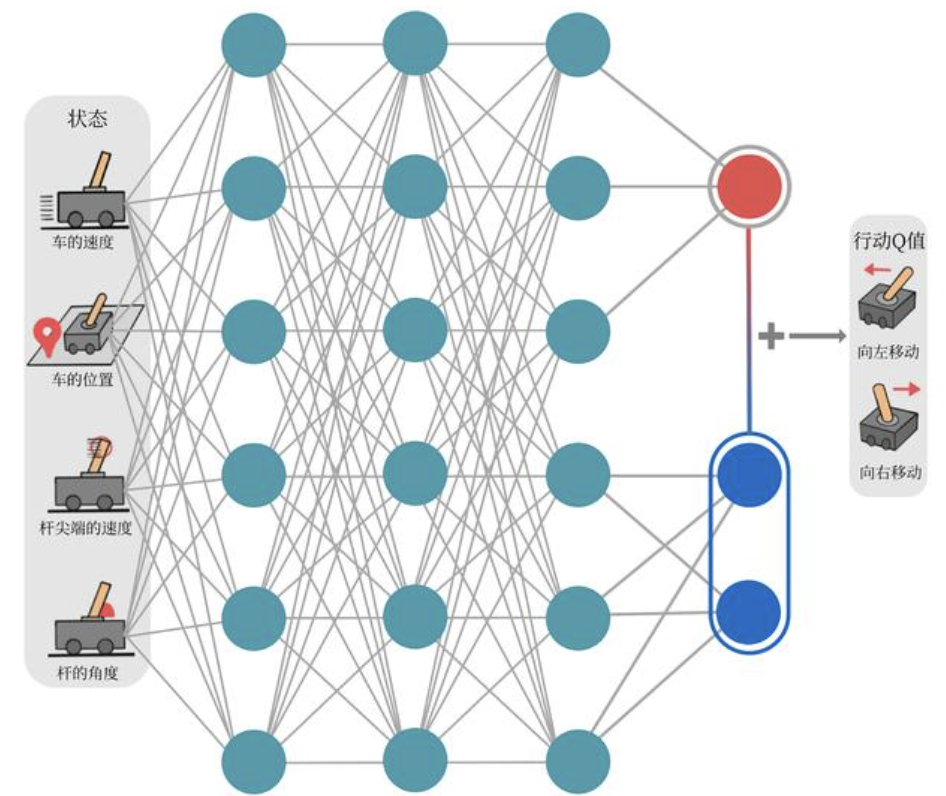
\includegraphics[width=0.618\linewidth]{pic/RL8/Dueling DQN.png}
    \caption{\label{fig:Dueling DQN}Dueling DQN 网络结构. 红色点表示状态价值函数输出, 蓝色点表示优势函数输出, 二者相加最后计算出动作价值.}
\end{figure}

这样分别建模状态价值函数和优势函数好处是强制智能体同时关注状态价值和不同动作的差异, 能更好处理与动作关联较小的状态. 

但是这样会有一个问题, 其 $V, A$ 的值不唯一. 例如对同一个 $Q$, 将 $V$ 加上一个常数 $C$, 将 $A$ 减去常数 $C$, 其 $Q$ 不变, 这样训练会不稳定. 为了解决这个问题, Dueling DQN 强制最优动作的优势函数实际输出位 0, 即
\begin{align*}
    Q_{\eta, \alpha, \beta} = V_{\eta, \alpha} (s) + A_{\eta, \beta} (s,a) - \max_{a'} A_{\eta, \beta}(s,a')
\end{align*} 
此时 $V(s)=\max_a Q(s,a)$ 可以确保 $V$ 的唯一性. 在实现过程中, 可以使用平均値代替最大化操作, 即
\begin{align*}
    Q_{\eta, \alpha, \beta} = V_{\eta, \alpha} (s) + A_{\eta, \beta} (s,a) - \frac{1}{|\AC|}\sum_{a'} A_{\eta, \beta} (s,a')
\end{align*}
此时 $V(s)=\frac{1}{|\AC|}\sum_{a'} A_{\eta, \beta} (s,a')$. 虽然不再满足贝尔曼最优方程, 但在实际应用中会更稳定. 

为什么 Dueling DQN 比 DQN 更好? 部分原因是其能更高效学习状态价值函数, 每次更新函数 $V$ 都会被更新, 且影响其他状态的 $Q$. 而传统 DQN 只会更新某个动作的 $Q$, 其他 $Q$ 可能不会更新. 所以 Dueling DQN 可以更加频繁且准确地学习状态价值函数. Dueling DQN 仍然用到了目标网络的优化技巧. 